\documentclass{article}

\usepackage{pgfplots}
\usepackage{tikz}
\usepackage{circuitikz}
\usepackage{amsmath}
\usepackage{graphicx}
\usepackage{float}
\usepackage{multirow}
\usepackage{array}
\usepackage{booktabs}
\usepackage{enumitem}
\usepackage{wrapfig}
\usepackage{pdfpages}
\usepackage{graphicx}
\usepackage{hyperref}
\usepackage{chngcntr}
\usetikzlibrary{positioning,arrows.meta,shapes.geometric}
\renewcommand{\tableautorefname}{Tabel}
\renewcommand{\sectionautorefname}{Afsnit}
\renewcommand{\subsectionautorefname}{Afsnit}
\renewcommand{\figureautorefname}{Figur}
\renewcommand{\figurename}{Figur}
\renewcommand{\contentsname}{Indholdsfortegnelse}
\counterwithout{figure}{section}
		\tikzstyle{startstop} = [
rectangle,
rounded corners,
minimum width=3cm,
minimum height=1cm,
text centered,
draw=black
]

\tikzstyle{process} = [
rectangle,
minimum width=3cm,
minimum height=1cm,
text centered,
draw=black
]

\tikzstyle{decision} = [
diamond,
minimum width=3cm,
minimum height=1cm,
text centered,
draw=black,
aspect=2
]

\tikzstyle{io} = [
trapezium,
trapezium left angle=70,
trapezium right angle=110,
minimum width=3cm,
minimum height=1cm,
text centered,
draw=black
]

\tikzstyle{arrow} = [
thick,
->,
>=Stealth
]
\title{Metaldetektor projekt \\Gruppe 1 \\s233986, s233988, s171678}

\begin{document}
\begin{titlepage}
	\centering
	
	{\LARGE \textbf{Metaldetektor projekt\\Gruppe 1}\par}
	\vspace{1cm}
	{\large 34621 \\ Electromagnetic sensors and digital signal processing \\ Danmarks Tekniske Universitet\par}
	\vspace{2cm}
	\begin{minipage}{0.3\textwidth}
		\centering
		\includegraphics[width=\linewidth,height=4cm,keepaspectratio,trim=1cm 1cm 1cm 1cm,clip]{Seb billede.png}\\
		\textbf{Sebastian Sørensen, s233986}
	\end{minipage}
	\hfill
	\begin{minipage}{0.3\textwidth}
		\centering
		\includegraphics[width=\linewidth,height=4cm,keepaspectratio,trim=1cm 1cm 1cm 1cm,clip]{Seb billede.png}\\
		\textbf{Oliver Holm, s233988}
	\end{minipage}
	\hfill
	\begin{minipage}{0.3\textwidth}
		\centering
		\includegraphics[width=\linewidth,height=4cm,keepaspectratio,trim=1cm 1cm 1cm 1cm,clip]{Bilal billede.png}\\
		\textbf{Bilal Alali, \newline s171678}
	\end{minipage}
	
	\vfill
	{\large \today}
	
\end{titlepage}
	\newpage
	\tableofcontents
	\newpage
\section{Introduktion}
	\begin{figure}[H]
		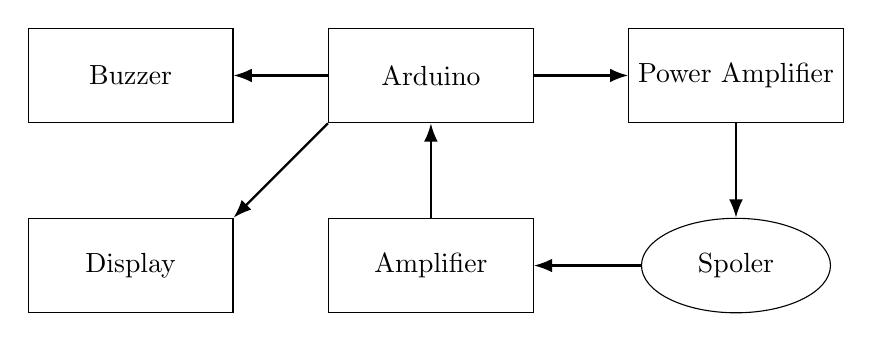
\begin{tikzpicture}[
			block/.style={
				draw,
				rectangle,
				minimum width=2.6cm,
				minimum height=1.2cm,
				align=center
			},
			io/.style={
				draw,
				ellipse,
				minimum width=2.4cm,
				minimum height=1.2cm,
				align=center
			},
			arrow/.style={
				->,
				thick,
				>=Latex
			}
			]
			
			% Nodes
			\node[block] (arduino) {Arduino};
			\node[block, left=1.2cm of arduino] (buzzer) {Buzzer};
			\node[block,below=1.2cm of buzzer] (display) {Display};
			\node[block, right=1.2cm of arduino] (pa) {Power Amplifier};
			\node[block, below=1.2cm of arduino] (amp) {Amplifier};
			\node[io,below=1.2cm of pa] (coils) {Spoler};
			
			% Arrows
			\draw[arrow] (arduino) -- (pa);
			\draw[arrow] (pa) -- (coils);
			\draw[arrow] (coils) -- (amp.east);
			\draw[arrow] (amp.north) -- (arduino.south);
			\draw[arrow] (arduino.south west) -- (display.north east);
			\draw[arrow] (arduino.west) -- (buzzer.east);
			
		\end{tikzpicture}
		\caption{Overordnet moduldiagram af systemet}
		\label{fig:ModuleDiagram}
	\end{figure}
\section{Analyse}
\section{Design}
	\subsection{Analogt design}
		\subsubsection{Energiberegninger}
		\subsubsection{Spoler og strømforstærkning}
			\begin{figure}[htbp]
				\centering
				\begin{circuitikz}[american,scale=0.8]
					% Q5
					\draw (3,3) node[npn,anchor=B,label={[align=left]right:{$Q_1$\\BC337-25}}] (Q5){};
					% Q6
					\draw (6,4) node[pnp,anchor=B,label={[align=left]right:{$Q_3$\\BC327-40}}](Q6){};
					% Q3
					\draw (6,7) node[npn,anchor=B,label={[align=left]right:{$Q_2$\\BC337-25}}](Q3){};
					% Q7
					\draw (8,3) node[npn,anchor=B,label={[align=left]right:{$Q_5$\\BC337-25}}] (Q7){};
					% Q4
					\draw (8,8) node[pnp,anchor=B,label={[align=left]right:{$Q_4$\\BC327-40}}] (Q4){};
					\draw	(0,0) node[ground]{} 
					to[sV, l={\shortstack{2\,kHz\\0--5\,V}}] (0,3)
					to [R=$10\text{k}\Omega$] ++(2,0)
					to [R=$10\text{k}\Omega$] ++(0,-3) to [short,-*]++(0,0);
					\draw (Q5.B) to [short,-*] (2,3);
					\draw (Q5.E) to [short,-*] ++(0,-2);
					\draw (Q5.C) to [short,-*] ++(0,1.5)
					to [short,-*] ++(1.95,0) -- (Q3.B) -- (Q6.B);
					\draw (Q5.C) -- ++(0,4) to [R=$10\text{k}\Omega$] ++(0,2.25) to [short,-*]++(0,0);
					\draw (Q3.C) to [short,-*] ++(0,0)  to [R=$10\text{k}\Omega$] ++(0,2.25) to 		[short,-*]++(0,0);
					\draw (Q4.E) to [short,-*]++(0,1.25);
					\draw (Q3.E) to [short,-*] ++(0,-0.8) to [short,-*]++(2,0);
					\draw (Q6.E) --++(0,1);
					\draw (Q7.C) to (Q4.C);
					\draw (Q6.C) to [short,-*]++(0,-0.05) to (Q7.B);
					\draw (Q6.C) --++(0,0) to [R=$10\text{k}\Omega$]++(0,-3) to [short,-*]++(0,0);
					\draw (Q4.B) --++(-1,0);
					\draw (Q7.E) to [short,-*]++(0,-2);
					\draw (11,0) to[D,l={\shortstack{$D_1$\\1N4148}}](11,3) to ++(0,2.25) 	coordinate(S1);
					\draw (S1) to [short,-*]++(0,0);
					\draw (S1) --++(-2.2,0);
					\draw (S1)  to [D,l={\shortstack{$D_2$\\1N4148}}]++(0,2) --++(0,3) to ++(-10,0) 	to 		[vsource=$9\text{V}$]++(0,-2) coordinate(9V-);
					\draw (S1) to [C=$1642\text{nF}$] ++(3,0) to [L=$3.855\text{mH}$]++(0,-2) 	to 		[R=$8.75\Omega$]++(0,-1.75) to ++(0,-1.5) to ++(-14,0);
					\draw (11,0) to [short,-*]++(0,0);
					\node[ground] at (9V-){};
				\end{circuitikz}
				\caption{Power amplifier kredsløb til at øge strømmen gennem TX-spolen.}
				\label{fig:PA}
			\end{figure}
		\subsubsection{Filtrering og forstærkning af spolesignal}
			\begin{figure}[htbp]
				\centering
				\begin{circuitikz}[american]
					\draw (0,0) node[ground]{} to [sV,l=$V_{RX coil}$] ++ (0,2) to [L=$11.75\text{mH}$] 	++(2,0) to [R=$41.9\Omega$]++(2,0)
					coordinate(N1) to [short,-*]++(0,0) to [C=$100\text{nF}$]++(0,-2) to 	[short,-*]++(0,0);
					\draw (N1) --++(2,0) coordinate (Vout) to [R=$50\text{k}\Omega$]++(0,-2) to 	[short,-*]++(0,0)coordinate(VR) to (0,0);
					\draw (Vout) to [short,-*]++(0,0) --++(2,0) to node[ocirc]{}++(0,0) 	coordinate(V+);
					\draw (VR) --++(2,0) to node[ocirc]{}++(0,0) coordinate(V-);
					\draw (V+) to [open,v=$V_{filtered}$] (V-);
				\end{circuitikz}
				\caption{Kredsløb til at filtrere støj væk ($\approx\frac{Fs}{2}=4\text{kHz}$) inden signalet bliver forstærket (som vist i \autoref{fig:OPAMP})}
				\label{fig:RXfilter}
			\end{figure}
				\begin{figure}[htbp]
					\centering
					\begin{circuitikz}[american]
						\draw (0,-2) node[ground]{} to [short,-*]++(0,0) to 		[vsourcesin,l=$V_{filtered}$]++(0,2)
						to [C=$1\mu\text{F}$]++(2,0) to [short,-*]++(0,0) coordinate(N1);
						\draw (N1) to [R=$100\text{k}\Omega$]++(0,-2) to [short,-*]++(0,0);
						\draw (N1) to [R=$100\text{k}\Omega$]++(0,4) to [short,-*]++(0,0) 	coordinate(N2) 	to [vsource,l=$5\text{V}$]++(0,2) --++(-2,0) coordinate(V-);%--++(0,-8) --++(10.8,0) coordinate(N5); % Linje til ground her
						\node[ground] at (V-){};
						\draw (0,-2) to ++(9,0) to node[ocirc]{}++(0,0) coordinate(Vout-);
						\draw (6,3.5) node[op amp,yscale=-1,label=south:MC6002] (opamp){};
						\draw (opamp.+) to (N2);
						\draw (opamp.-) to [short,-*]++(0,-1) coordinate(N3) to 		[R=$14\text{k}\Omega$]++(0,-2) to [C=$1\mu\text{F}$]++(0,-2) to [short,-*]++(0,0);
						\draw (N3) to [R=$90\text{k}\Omega$] ++(3,0) to [short,-*]++(0,1.5) 		coordinate(Vo);
						\draw (Vo) to (opamp.out);
						\draw (Vo) --++(1.25,0) to node[ocirc]{}++(0,0) coordinate(Vout+);
						\draw (Vout+) to [open,v=$V_{out}$](Vout-);
						%	\draw (Vo) --++(1,0) to [open,v^=$V_{out}$](N5);
					\end{circuitikz}
					\caption{Kredsløb til at forstærke den filtrerede spænding fra RX-spolen op, inden det læses ind i MCU ADC'en.}
					\label{fig:OPAMP}
				\end{figure}
	\subsection{Digitalt design}
		\subsubsection{Moduldiagram og introduktion}
			\begin{figure}[H]
				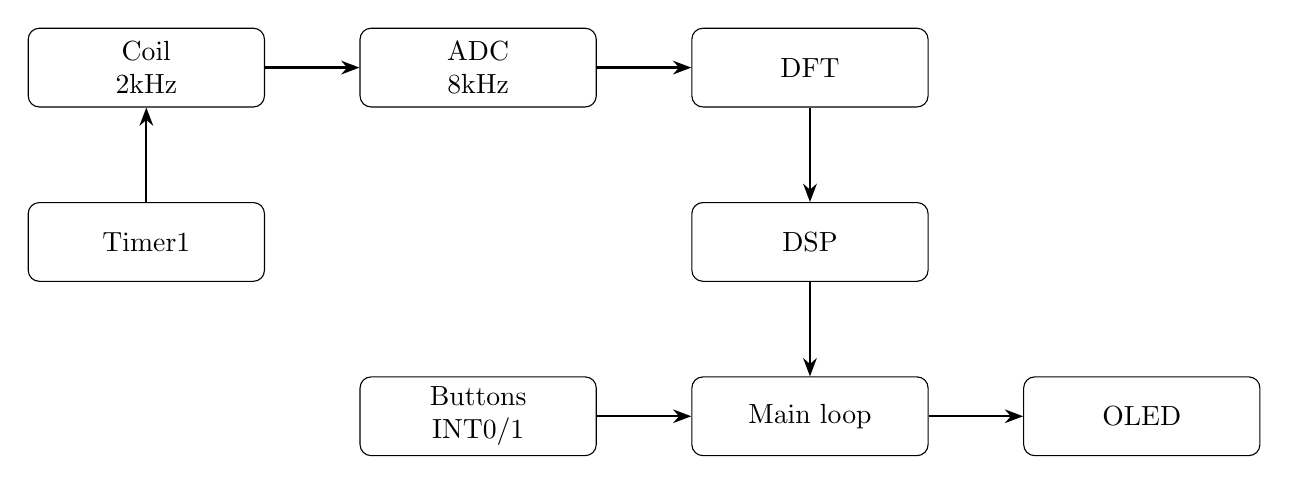
\begin{tikzpicture}
					%Nodes
					\node[startstop,align=center] (coil) {Coil\\2kHz};
					\node[startstop,align=center,right=1.2cm of coil] (adc) {ADC\\8kHz};
					\node[startstop,right=1.2cm of adc] (dft) {DFT};
					\node[startstop,below=1.2cm of dft] (dsp) {DSP};
					\node[startstop,below=1.2cm of coil] (timer1) {Timer1};
					\node[startstop,below=1.2cm of dsp] (main) {Main loop};
					\node[startstop,right=1.2cm of main] (oled) {OLED};
					\node[startstop,align=center,left=1.2cm of main] (buttons) {Buttons\\INT0/1};
					%Arrows
					\draw[arrow] (coil.east) -- (adc.west);
					\draw[arrow] (adc.east) -- (dft.west);
					\draw[arrow] (dft.south) -- (dsp.north);
					\draw[arrow] (timer1.north) -- (coil.south);
					\draw[arrow] (dsp.south) -- (main.north);
					\draw[arrow] (buttons.east) -- (main.west);
					\draw[arrow] (main.east) -- (oled.west);
				\end{tikzpicture}
				\caption{Overordnet moduldiagram af systemet}
				\label{fig:DigitalModulDiagram}
			\end{figure}
		\subsubsection{Brugerinteraktion}
		\subsubsection{DFT algoritme og sampling}
		\begin{figure}[H]
			\centering
			\includegraphics[width=0.5\linewidth]{"DFT plot"}
			\caption{Grafisk illustration over princippet bag DFT-algoritmen. Ved at vælge $F_d=\frac{F_s}{4}$, undgår vi at lave komplicerede komplekse beregninger.}
			\label{fig:dft-plot}
		\end{figure}
		\subsubsection{Tilstandsmaskine}
		\subsubsection{Digital signal behandling}

\section{Implementering og test}
\end{document}